% SASYR 2025 - Template based on:
% samplepaper.tex, a sample chapter demonstrating the
% LLNCS macro package for Springer Computer Science proceedings;
% Version 2.20 of 2017/10/04
%
\documentclass[runningheads]{llncs}
%
\usepackage{graphicx}
\usepackage{lipsum}
\usepackage{url}
\usepackage[utf8]{inputenc} % allow utf-8 input
\usepackage[T1]{fontenc}    % use 8-bit T1 fonts
\usepackage{hyperref}       % hyperlinks
\usepackage{url}            % simple URL typesetting
\usepackage{booktabs}       % professional-quality tables
\usepackage{amsfonts}       % blackboard math symbols
\usepackage{nicefrac}       % compact symbols for 1/2, etc.
\usepackage{microtype}      % microtypography
\usepackage{xcolor}         % colors
\usepackage{graphicx}       % addtional package for show figures
% Used for displaying a sample figure. If possible, figure files should
% be included in EPS format.
%
% If you use the hyperref package, please uncomment the following line
% to display URLs in blue roman font according to Springer's eBook style:
% \renewcommand\UrlFont{\color{blue}\rmfamily}

\begin{document}
%
\title{Case Study}
%
%\titlerunning{Abbreviated paper title}
% If the paper title is too long for the running head, you can set
% an abbreviated paper title here
%
\author{Ali Doğukan Seven \and
Yisong Tang\ \and
Karel Štícha 
}
%
% First names are abbreviated in the running head.
% If there are more than two authors, 'et al.' is used.
%
\institute{Johannes Kepler University \\
}
%
\maketitle              % typeset the header of the contribution
%
%
%
%
\section{The Case Study}
\subsection{ A) Identify Similarities and Differences}

Temporal Differences: In 44534, clear sounds were not annotated, such as barking and car noise (00:06–00:20). Annotations in 623746 did not include or oversimplified repeating synthetic sounds and the full utterance from the woman (00:03-00:12). 

Textual Differences: Nearly all of the major sounds, such as flute melodies, barking, and singing, were disregarded. The emotional tone of the woman's voice (e.g., excitement) was not noted. (Unclear whether the dogs were aggressive due to distance.) 

Similarity: Both annotators could have been subjected to listener-related biases toward the primary sounds, often missing background events entirely, thus resulting in different interpretations of the task.
\subsubsection{B) Assessing Audio Metadata} Only two levels of
Such annotations only mention the panpipe melody in 44534 and rattle one corresponding keyword in the metadata. Other metadata, terms such as "shout," "salesman," among others, remain unrepresented, and key sounds such as dog barks and car noises do not feature at all.

Annotation 623746 reduces the audio to the simplest terms: "a woman says one word," which does not represent the actual singing or the synthetic background sounds. Although the metadata suggest an emergency context ("alarm," "fire"), the audio does not provide that strong support: Thuss, language barrier made it hard to distinguish if the written metadata true or the one I wrote.

\subsubsection{C) Assesing Text Annotation}

In both recordings, weak temporal and textual annotations can be observed. For example, in recording 44534, the timing of car sounds, dog barks, and the different flute melodies is neglected. In recording 623746, various phases of sound (synthetic, speech, music) are not tagged (this part may be ignored). Textually, the annotations in both cases are too vague as background sounds and emotion cues are disregarded. Therefore, it can be said that the annotations do not meet the desired requirements.



%%%%%%%Part 2 Annotation Quality Start%%%%%%%%%

\section{Annotation Quality}

\subsubsection{(a) Precision of temporal annotations}
We assessed the precision of temporal annotations by analyzing the duration of overlapping annotations (Table~\ref{tab:dur}). The standard deviation was approximately 10 seconds, and the inter-quartile range exceeded 20 seconds, suggesting significant variability.
However, annotators agreed on the number of distinct sound events in 94.7\% of cases, indicating consistency in event identification despite differences in duration. 

\begin{table}[h]
    \caption{Summary Statistics of Duration of Overlapping Annotations.}
    \label{tab:dur}
    \centering
    \begin{tabular}{lcl}
        \toprule
        Statistic & Duration (in seconds) \\ \midrule
        Mean            & 10.694948 \\
        Std             & 10.100707 \\
        Min             & 0.052521 \\
        25\%            & 1.343494 \\
        50\%            & 5.799818 \\
        75\%            & 20.679048 \\ 
        Max             & 30.044718 \\ \bottomrule
    \end{tabular}
\end{table}


\subsubsection{(b) Similarity of textual annotations}
We measured textual similarity in overlapping regions using annotation length and cosine similarity. Text length varied significantly, with a standard deviation of 4.33 words.
Cosine similarity analysis (Table~\ref{tab:cos}) revealed low agreement among annotators, with a mean of 0.06 and an inter-quartile range from -0.03 to 0.14. This suggests that descriptions often differed substantially, and in some cases, even opposed each other.  

\begin{table}[h]
    \caption{Summary Statistics of Cosine Similarity of Overlapping Annotations.}
    \label{tab:cos}
    \centering
    \begin{tabular}{lcl}
        \toprule
        Statistic & Cosine Similarity \\ \midrule
        Mean            & 0.063015 \\
        Std             & 0.144213 \\
        Min             & -0.357656 \\
        25\%            & -0.032708 \\
        50\%            & 0.049751 \\
        75\%            & 0.140056 \\ 
        Max             & 0.848671 \\ \bottomrule
    \end{tabular}
\end{table}

\subsubsection{(c) Frequency of annotations and sound events}
Each sound file contained an average of 3.99 annotations and 3.72 distinct sound events, with a minimum of 1. The minimum is reasonable considering that some files may contain a single continuous sound.

\subsubsection{(d) Detail of annotations}
The level of detail in individual annotations varied significantly. The distribution of annotation lengths displayed in Figure~\ref{fig:len} is positively skewed, suggesting that most descriptions were brief, with a median of 7 words.

\begin{figure}[h]
    \centering
    %Elbow+Silhouette plot
    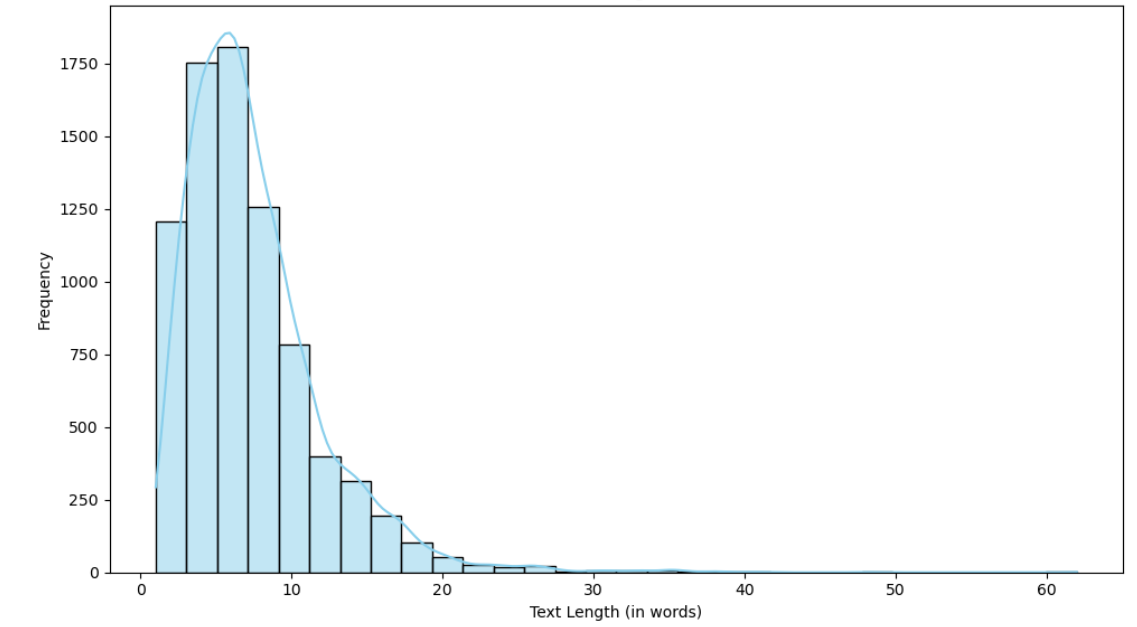
\includegraphics[width=.55\linewidth]{distribution_of_text_lengths.PNG}
    \caption{Distribution of Text Lengths in Annotations.}
    \label{fig:len}
\end{figure}

\subsubsection{(d) Inconsistencies and outliers}
No technical errors were found (e.g., offsets preceding onsets or zero-duration annotations) and these checks could be implemented automatically.
Regarding the content, annotations with zero or very short lengths (<2 words) may be considered inadequate. However, using statistical outlier detection (e.g., IQR) may be overly limiting and could flag valid annotations.


%%%%%%%Part 2 Annotation Quality Finish%%%%%%%%%

%%%%%%%Part 3 Audio Features Start%%%%%%%%%

\section{Audio Features}

\subsubsection{(a) Feature choice and dimension cut}
We checked the 13 frame features in each \texttt{.npz} file. Some were almost the same or did not add much information, for example \texttt{power} is almost equal to \texttt{energy}. We also dropped \texttt{mfcc\_delta2} and \texttt{flatness}. The nine groups we kept are in Table~\ref{tab:feat}.

We normalised every frame with a \texttt{StandardScaler}. Then we ran PCA. The first PCA keeps \textbf{95.4\%} of the variance with 62 components (Figure~\ref{fig:pca}). A second PCA cuts it to 50 dimensions.

\begin{table}[h]
    \caption{Retained frame feature groups (total $140$\,dims).}
    \label{tab:feat}
    \centering
    \begin{tabular}{lcl}
        \toprule
        Group & \#dims & Reason \\ \midrule
        Mel spectrogram            & 64 & dense spectral envelope \\
        MFCC + $\Delta$            & 64 & static \& dynamic timbre \\
        Spectral contrast          & 7  & noise vs. harmonic      \\
        Centroid, bandwidth, flux  & 3  & brightness / variation   \\
        Energy, ZCR                & 2  & loudness / noisiness     \\ \bottomrule
    \end{tabular}
\end{table}

\begin{figure}[h]
    \centering
    % PCA cumulative variance plot
    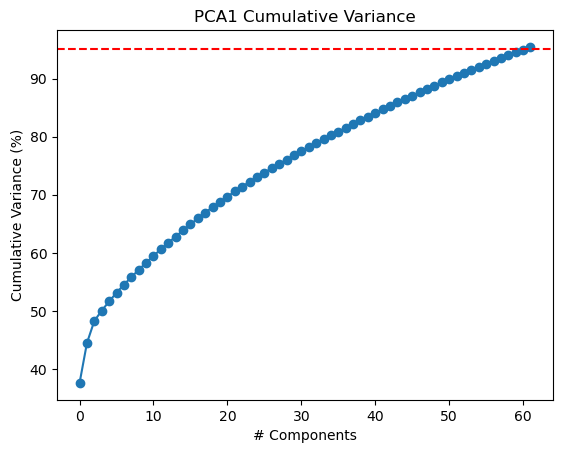
\includegraphics[width=.55\linewidth]{figs_tang/03_pca_cumulative_variance.png}
    \caption{Cumulative variance curve; the red dashed line marks 95\%.}
    \label{fig:pca}
\end{figure}

\subsubsection{(b) Fixed-length vectors for each region}
For every labelled segment $(t_\text{on}, t_\text{off})$ and the matching silent part, we make one 50‑D vector. We first project every frame through the two PCAs and then take the mean:
\[
\mathbf v = \frac{1}{N}\sum_{t=i_0}^{i_1-1}
\mathrm{PCA}_2(\mathrm{PCA}_1(\mathrm{Scaler}(\mathbf f_t))).
\]
This gives \textbf{51\,966} vectors: 35\,723 from events and 16\,243 from silence.

\subsubsection{(c) Clustering and silence check}
We tried $k$‑Means with $k=4\ldots30$. The best silhouette score (0.18) is at $k=4$ (Figure~\ref{fig:elbow}). Table~\ref{tab:cluster} shows the four clusters. Cluster~2 holds \textbf{84\%} of the silence vectors; most of the rest of the silence is in cluster~3.

\begin{figure}[h]
    \centering
    %Elbow+Silhouette plot
    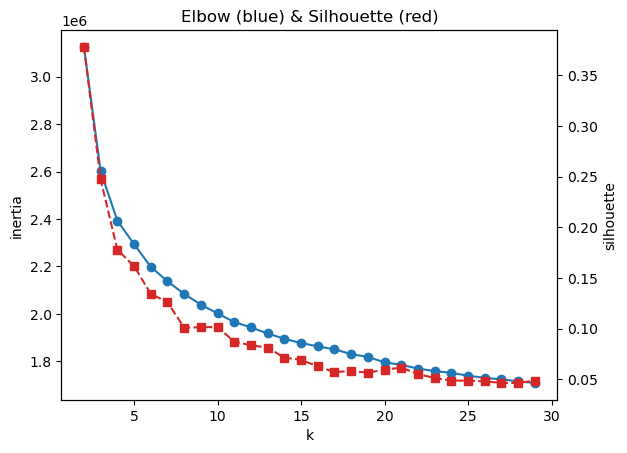
\includegraphics[width=.55\linewidth]{figs_tang/03_elbow_silhouette.png}
    \caption{Elbow curve (blue) and silhouette score (red) for different $k$.}
    \label{fig:elbow}
\end{figure}

\begin{table}[h]
    \caption{Cluster statistics for $k=4$.}
    \label{tab:cluster}
    \centering
    \begin{tabular}{cccc}
        \toprule
        id & size & silence (\%) & perceptual label \\ \midrule
        0 & 17\,944 & 19 & vehicle / rumble \\
        1 & 15\,745 & 11 & sharp metallic hits \\
        \textbf{2} & 6\,447 & \textbf{84} & near‑silence \\
        3 & 11\,830 & 47 & diffuse ambience \\ \bottomrule
    \end{tabular}
\end{table}

\begin{figure}[h]
    \centering
    % PCA scatter plots
    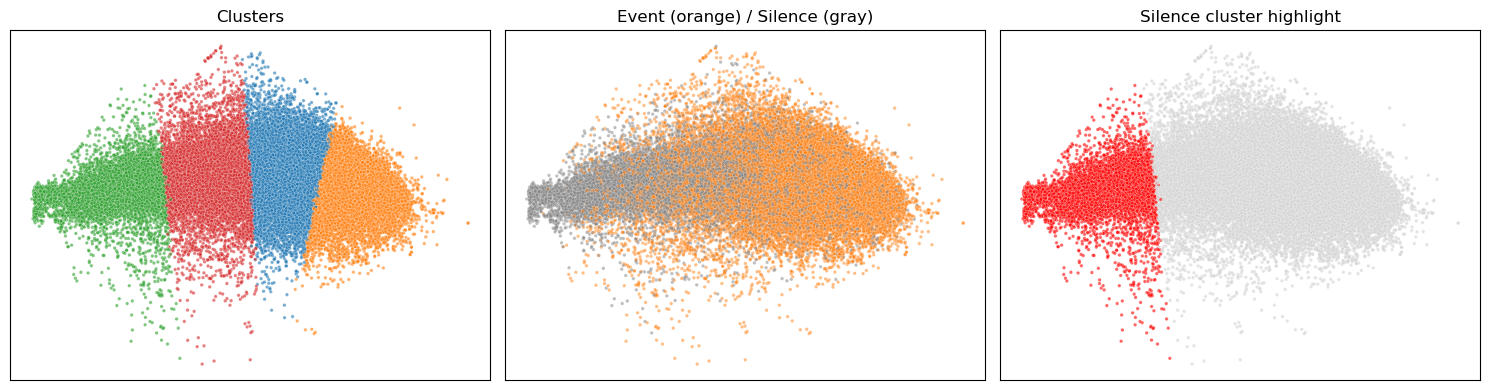
\includegraphics[width=.45\linewidth]{figs_tang/03_pca_clusters.png}
    \caption{Left: clusters in 2‑D PCA space; Right: event (orange) vs. silence (grey).}
    \label{fig:pca_scatter}
\end{figure}

These four clusters already split silence and three big sound types. They work as rough labels for training the detector later.

%%%%%%%Part 3 Audio Features Finish%%%%%%%%%

%%%%%%% Part 4 Text Features Start %%%%%%%%%

\section{Text Features}

\subsubsection{(a) Picking $k$ for text embeddings}
We load 35\,826 sentence‑transformer embeddings (1\,024‑D, unit norm). A PCA that keeps 90\,\% of the variance shrinks them to 100 dimensions. We then run $k$‑Means for $k=5\ldots20$. The silhouette curve in Figure~\ref{fig:text_silhouette} reaches a local maximum at $k=15$ ($s=0.071$), so we choose \textbf{$k=15$}. The t‑SNE plots in Figure~\ref{fig:text_tsne} show cleaner colour islands for $k=15$ than for $k=11$.

\begin{figure}[h]
  \centering
  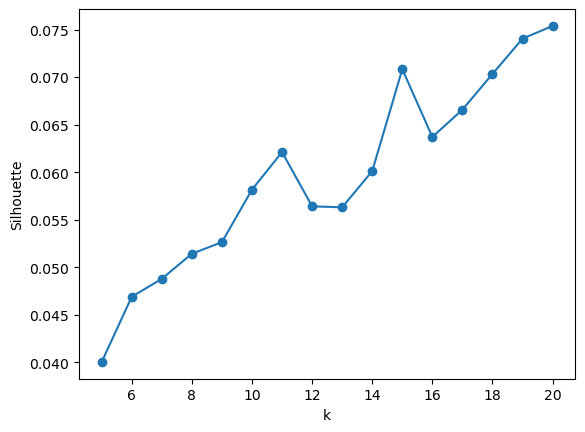
\includegraphics[width=.55\linewidth]{figs_tang/04_silhouette_k.png}
  \caption{Silhouette over $k=5\ldots20$ (text embeddings).}
  \label{fig:text_silhouette}
\end{figure}

\begin{figure}[h]
  \centering
  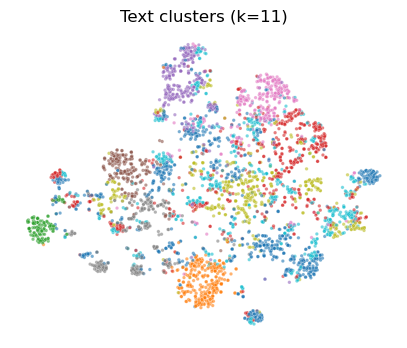
\includegraphics[width=.45\linewidth]{figs_tang/04_text_cluster11.png}\hfill
  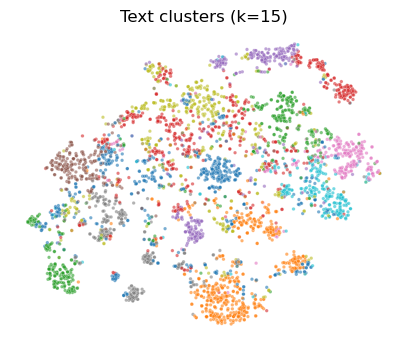
\includegraphics[width=.45\linewidth]{figs_tang/04_text_cluster15.png}
  \caption{t‑SNE colour map of text clusters for $k=11$ (left) and $k=15$ (right).}
  \label{fig:text_tsne}
\end{figure}

\subsubsection{(b) Themes of the 15 clusters}
We listen to five random clips in every cluster. Table~\ref{tab:text_themes} lists the main sound we hear: bells (\texttt{C0}), sirens or buzzing (\texttt{C1}), dogs or birds (\texttt{C2}), water or rain (\texttt{C3}), etc. This quick check tells us the clusters are semantically meaningful.

\begin{table}[h]
  \caption{Manual auditory label of the 15 text clusters.}
  \label{tab:text_themes}
  \centering
  \small
  \begin{tabular}{cl}
    \toprule
    Cluster & Dominant sound theme \\ \midrule
    0 & bell sound \\
    1 & buzzing sound / siren \\
    2 & dogs or birds \\
    3 & water / rain \\
    4 & repeating mechanical sound \\
    5 & vocal sound \\
    6 & engine / vehicle \\
    7 & high‑pitched vocal (kitten / child) \\
    8 & high‑pitched noise / drill \\
    9 & high‑level ambience \\
    10 & hissing / scratching \\
    11 & generic animal farm / birds \\
    12 & high‑pitched repeating motor \\
    13 & rhythmic footsteps / cheering \\
    14 & low‑level ambience / jazz \\
    \bottomrule
  \end{tabular}
\end{table}

\subsubsection{(c) Dog \& cat tagging rule}
A simple rule—regex \texttt{(bark$|$woof$|$puppy)} or \texttt{(meow$|$purr$|$kitten)} plus cosine similarity $>0.35$ to class prototypes—finds \textbf{1\,483 dog} and \textbf{731 cat} tags. The entropy for both is 0.073, meaning over 80\,\% of each class sits in only two clusters. Figure~\ref{fig:dogcat_tsne} shows how tightly these points group in t‑SNE space.

\begin{figure}[h]
  \centering
  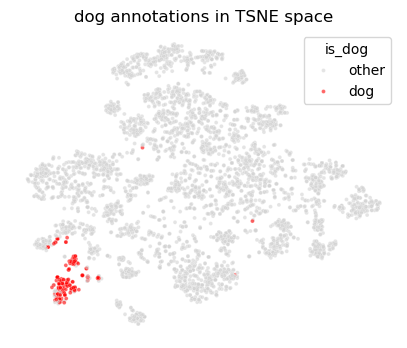
\includegraphics[width=.42\linewidth]{figs_tang/04_dog_annotations_in_tsne_space.png}\hfill
  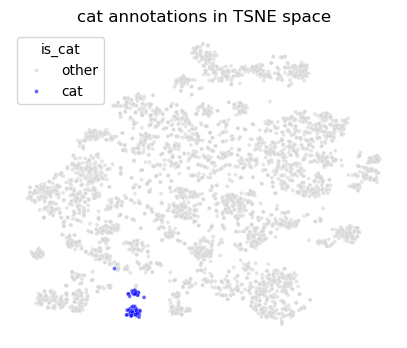
\includegraphics[width=.42\linewidth]{figs_tang/04_cat_annotations_in_tsne_space.png}
  \caption{Dog (left) and cat (right) annotations highlighted in t‑SNE space.}
  \label{fig:dogcat_tsne}
\end{figure}

\subsubsection{(d) Linking text and audio clusters}
The 51\,966 audio region vectors were clustered into four groups (see Section~3c). After matching by \texttt{(filename, onset, offset)} rounded to 1 ms we get 35\,552 event pairs. Four very small text clusters ($<0.3$\,\% each) have no audio match, so their rows are zero in Figure~\ref{fig:text_audio_heat}. The heatmap shows clear links—bells map to audio 0, speech to 1, animal calls to 2, water/ambience to 3. The Normalised Mutual Information is \textbf{NMI = 0.28}.

\begin{figure}[h]
  \centering
  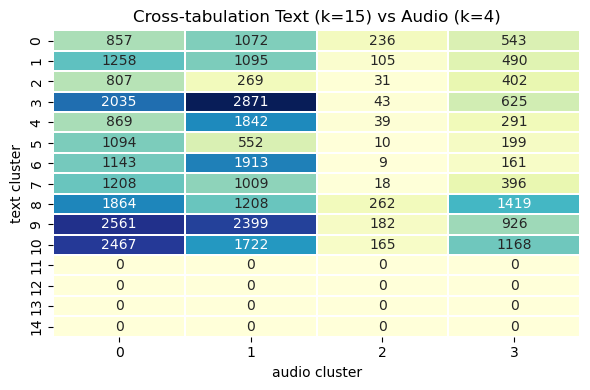
\includegraphics[width=.7\linewidth]{figs_tang/04_text_audio_heatmap_k15.png}
  \caption{Cross‑tabulation of text clusters ($k=15$) vs. audio clusters ($k=4$). Rows 11–14 are empty because those text clusters contain only sub‑frame annotations without audio features.}
  \label{fig:text_audio_heat}
\end{figure}

\paragraph{Take‑aways.} Text embeddings form 15 clear semantic clusters. The dog/cat rule confirms tight grouping. An NMI of 0.28 suggests a moderate but useful link between text and audio spaces, enough to transfer weak labels between them.

%%%%%%% Part 4 Text Features Finish %%%%%%%%%

\section{Conclusions} 
 The dataset is of limited utility for general-purpose sound event detection, especially in determining whether or not an event occurred. Its high variation regarding the lengths of time events are labeled, combined with vague textual descriptions, makes it unreliable for using the dataset for more specific purposes.

Biases include a fondness for short annotations, mixed wording, and an absence of attendance with background or emotional sounds. One-word annotations are common, but they are often uninformative, limiting the usefulness of the dataset.
\end{document}